\documentclass[addpoints,10pt]{exam}

% Page configurations
\title{ME: MECHANICAL ENGINEERING}
\usepackage[a4paper,bottom=1in,top=1in]{geometry}
\usepackage{amsmath}
\usepackage{tikz}
\usetikzlibrary{arrows}
% \usetikzlibrary{decorations.markings}
\graphicspath{{images/}}

% Header and footer
\pagestyle{headandfoot}
\headrule
\header{2008}{}{MAIN PAPER - ME}
\footrule
\footer{ME}{}{\thepage/\numpages}

\renewcommand{\thequestion}{Q.\arabic{question}}
\renewcommand{\thechoice}{(\Alph{choice})}
\renewcommand{\choicelabel}{\thechoice}

\begin{document}
\begin{center}
    \Large
    \textbf{ME: MECHANICAL ENGINEERING}
\end{center}

\textit{Duration} : Three hours
\hfill
\textit{Maximum Marks} : 150
\\\\
\textbf{Read the following instructions carefully}
\begin{enumerate}
    \item This question paper contains \textbf{24} printed pages including pages for rough work. Please check all pages and report discrepancy, if any.
    \item Write your registration number, your name and name of the examination centre at the specified locations on the right half of the ORS.
    \item Using HB pencil, darken the appropriate bubble under each digit of your registration number and the letters corresponding to your paper code.
    \item All the questions in this question paper are of objective type.
    \item Questions must be answered on \textbf{O}bjective \textbf{R}esponse \textbf{S}heet (\textbf{ORS}) by darkening the appropriate bubble (marked A, B, C, D) using HB pencil against the question number on the left hand side of the ORS. \textbf{Each question has only one correct answer}. In case you wish to change an answer, erase the old answer completely. More than one answer bubbled against a question will be treated as a wrong answer.
    \item Questions 1 through 20 are 1-mark questions and questions 21 through 85 are 2-mark questions.
    \item Questions 71 through 73 is one set of common data questions. The question pairs (76, 77), (78, 79), (80, 81), (82, 83) and (84, 85) are questions with linked answers. The answer to the second question of the above pairs will depend on the answer to the first question of the pair. If the first question in the linked pair is wrongly answered or is un-attempted, then the answer to the second question will not be evaluated.
    \item Unattempted questions will carry zero marks.
    \item \textbf{NEGATIVE MARKING}: For Q.1 to Q.20, 0.25 mark will be deducted for each wrong answer. For Q.21 to Q.75, 0.5 mark will be deducted for each wrong answer. For the pairs of questions with linked answers, there will be negative marks only for wrong answer to the first question, i.e. for Q.76, Q.78, Q.80, Q.82 and Q.84, 0.5 mark will be deducted for each wrong answer. There is no negative marking for Q.77, Q.79, Q.81, Q.83 and Q.85.
    \item Calculator \textbf{without data connectivity} is allowed in the examination hall.
    \item Charts, graph sheets and tables are NOT allowed in the examination hall.
    \item Rough work can be done on the question paper itself. Additional blank pages are given at the end of the question paper for rough work.
\end{enumerate}
\newpage

\large\textbf{Q.1 -- Q.20 carry one mark each.}\\
\begin{questions}

    \question In the Taylor series expansion of $e^x$ about x=2, the coefficient of $(x-2)^4$ is

    \begin{oneparchoices}
        \choice $\frac{1}{4!}$
        \choice $\frac{2^4}{4!}$
        \choice $\frac{e^2}{4!}$
        \choice $\frac{e^4}{4!}$
    \end{oneparchoices}

    \question Given that $\ddot{x} + 3x = 0$, and $x(0)=1$, $\dot{x}(0)=(0)$, what is $x(1)$?

    \begin{oneparchoices}
        \choice $-0.99$
        \choice $-0.16$
        \choice $0.16$
        \choice $0.99$
    \end{oneparchoices}

    \question The value of $\lim{x\rightarrow8} \frac{x^{\frac{1}{3}}-2}{(x-8)}$ is

    \begin{oneparchoices}
        \choice $\frac{1}{16}$
        \choice $\frac{1}{12}$
        \choice $\frac{1}{8}$
        \choice $\frac{1}{4!}$
    \end{oneparchoices}

    \question A coin is tossed 4 times. What is the probability of getting heads exactly 3 times?

    \begin{oneparchoices}
        \choice $\frac{1}{4}$
        \choice $\frac{3}{8}$
        \choice $\frac{1}{2}$
        \choice $\frac{3}{4}$
    \end{oneparchoices}

    \question The matrix $\begin{bmatrix}
            1 & 2 & 4 \\
            3 & 0 & 6 \\
            1 & 1 & p
        \end{bmatrix}$ has one eigenvalue equal to 3. The sum of the other two eigenvalues is

    \begin{oneparchoices}
        \choice $p$
        \choice $p-1$
        \choice $p-2$
        \choice $p-3$
    \end{oneparchoices}

    \question The divergence of the vector field $(x-y)\hat{i} + (y-x)\hat{j} + (x+y+z)\hat{k}$ is

    \begin{oneparchoices}
        \choice $0$
        \choice $1$
        \choice $2$
        \choice $3$
    \end{oneparchoices}

    \question The transverse shear stress acting in a beam of rectangular cross-section, subjected to a transverse shear load, is

    \begin{choices}
        \choice variable with maximum at the bottom of the beam
        \choice variable with maximum at the top of the beam
        \choice uniform
        \choice variable with maximum on the neutral axis
    \end{choices}

    \question A rod of length $L$ and diameter $D$ is subjected to a tensile load $P$. Which of the following is sufficient to calculate the resulting change in diameter?

    \begin{choices}
        \choice Young's modulus
        \choice Shear modulus
        \choice Poisson's ratio
        \choice Both Young's modulus and shear modulus
    \end{choices}

    \question A straight rod of length $L(t)$, hinged at one end and freely extensible at the other end, rotates through an angle $\theta(t)$ about the hinge. At time $t$, $L(t)=1$ m, $\dot{L}(t)=1$ m/s, $\theta(t)=\frac{\pi}{4}$rad and $\dot{\theta}(t)=1$ rad/s. The magnitude of the velocity at the other end of the rod is

    \begin{oneparchoices}
        \choice $1$m/s
        \choice $\sqrt{2}$m/s
        \choice $\sqrt{3}$m/s
        \choice $2$m/s
    \end{oneparchoices}
    \pagebreak

    \question A cantilever type gate hinged at Q is shown in the figure. P and R are the centers of gravity of the cantilever part and the counterweight respectively. The mass of the cantilever part is 75 kg. The mass of the coutnerweight, for static balance, is

    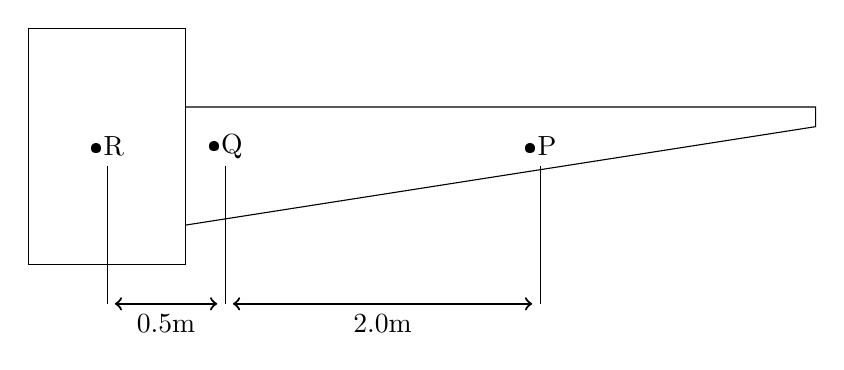
\begin{tikzpicture}
        \draw (0,0) rectangle (2,3);
        \node at (1,1.5) {•R};
        \draw[very thin] (1,1.25) -- (1,-0.5);
        \draw (2,2) -- (10,2) -- (10,1.75) -- (2,0.5);
        \node at (2.5,1.5) {•Q};
        \draw[very thin] (2.5,1.25) -- (2.5,-0.5);
        \node at (6.5,1.5) {•P};
        \draw[very thin] (6.5,1.25) -- (6.5,-0.5);
        \draw[thick, <->] (1.1,-0.5) -- (2.4,-0.5);
        \draw[thick, <->] (2.6,-0.5) -- (6.4,-0.5);
        \node at (1.75,-0.75) {0.5m};
        \node at (4.5,-0.75) {2.0m};
    \end{tikzpicture}

    \begin{oneparchoices}
        \choice 75kg
        \choice 150kg
        \choice 225kg
        \choice 300kg
    \end{oneparchoices}

    \question A planar mechanism has 8 links and 10 rotary joints. The number of degrees of freedom of the mechanism, using Greubler's criterion, is

    \begin{oneparchoices}
        \choice $0$
        \choice $1$
        \choice $2$
        \choice $3$
    \end{oneparchoices}

    \question An axial residual compressive stress due to a manufacturing process is present on the outer surface of a rotating shaft subjected to bending. Under a given bending load, the fatigue life of the shaft in the presence of residual compressive stress is

    \begin{choices}
        \choice decreased
        \choice increased or decreased, depending on the external bending load
        \choice neither decreased nor increased
        \choice increased
    \end{choices}

    \question 2 moles of oxygen are mixed adiabatically with another 2 moles of oxygen in a mixing chamber, so that the final total pressure and temperature of the mixture become same as those of the individual constituents at their intial states. The universal gas constant is given as $R$. The change in entropy due to mixing, per mole of oxygen, is given by

    \begin{oneparchoices}
        \choice $-R \ln2$
        \choice $0$
        \choice $R \ln 2$
        \choice $R\ln4$
    \end{oneparchoices}

    \question For flow of liquid over a heated plate, the following fluid properties are known:\\
    viscosity = 0.001 Pa.s ; specific heat constant pressure = 1kJ/kg.K ;\\
    thermal conductivity = 1 W/m.K.\\
    The hydrodynamic boundary layer thickness at a specified location on the plate is 1 mm. The thermal boundary layer thickness at the same location is

    \begin{oneparchoices}
        \choice 0.001 mm
        \choice 0.01 mm
        \choice 1 mm
        \choice 1000 mm
    \end{oneparchoices}

    \pagebreak

    \question For the continuity equation given by $\bar{\nabla}\cdot\bar{V} = 0$ to be valid, where $\bar{V}$ is the velocity vector, which one of the following is a necessary condition?

    \begin{choices}
        \choice steady flow
        \choice irrotational flow
        \choice inviscid flow
        \choice incompressible flow
    \end{choices}

    \question Which one of the following is NOT a necessary assumption for the air-standard Otto cycle?

    \begin{choices}
        \choice All processes are both internally as well as externally reversible.
        \choice Intake and exhaust processes are constant volume heat rejection processes.
        \choice The combustion process is a constant volume heat addition process.
        \choice The working fluid is an ideal gas with constant specific heats.
    \end{choices}

    \question In an M/M/1 queueing system, the number of arrivals in an interval of length $T$ is a Poisson random variable (i.e. the probability of there being $n$ arrivals in an interval of length $T$ is $\frac{e^{-\lambda T}(\lambda T)^n}{n!}$). The probability density function $f(t)$ of the inter-arrival time is given by

    \begin{oneparchoices}
        \choice $\lambda^2(e^{-\lambda^2t})$
        \choice $\frac{e^{-\lambda^2t}}{\lambda^2}$
        \choice $\lambda e^{-\lambda t}$
        \choice $\frac{e^{-\lambda t}}{\lambda}$
    \end{oneparchoices}

    \question A set of 5 jobs is to be processed on a single machine. The processing time (in days) is given in the table below. The holding cost for each job is Rs. $K$ per day.\\
    \begin{center}
    \begin{tabular}{|l|l|}
        \hline
        \textbf{Job} & \textbf{Processing time} \\
        \hline
        P & 5 \\\hline
        Q & 2 \\\hline
        R & 3 \\\hline
        S & 2 \\\hline
        T & 1 \\\hline
    \end{tabular}
    \end{center}
    A schedule that minimizes the total inventory cost is

    \begin{oneparchoices}
        \choice T-S-Q-R-P
        \choice P-R-S-Q-T\\
        \choice T-R-S-Q-P
        \choice P-Q-R-S-T
    \end{oneparchoices}

    \question For generating a Coon's surface we require
    \begin{choices}
        \choice a set of grid points on the surface
        \choice a set of grid control points
        \choice four bounding curves defining the surface
        \choice two bounding curves and a set of grid control points
    \end{choices}

    \question Internal gear cutting operation can be performed by
    \begin{choices}
        \choice milling
        \choice shaping with rack cutter
        \choice shaping with pinion cutter
        \choice hobbing
    \end{choices}
\end{questions}
\pagebreak
\large\textbf{Q.21 -- Q.75 carry two marks each.}\\
\begin{questions}
    \question Consider the shaded triangular region $P$ shown in the figure. What is $\iint\limits_P xy\mathrm{d}x\mathrm{d}y$?
    \begin{center}
        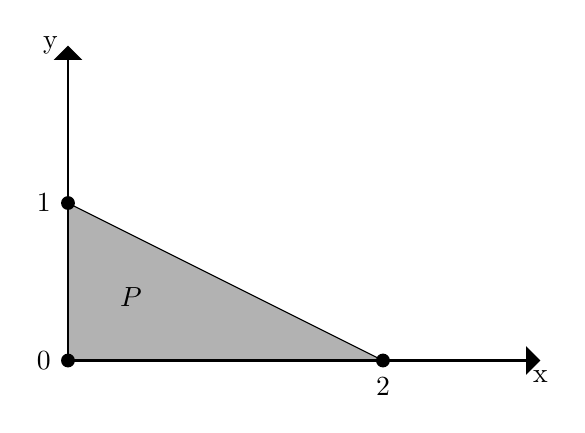
\begin{tikzpicture}[scale=2]
            \centering
            \fill[black!30!white] (0,0) -- (2,0) -- (0,1) -- cycle;
            \node at (0.4,0.4) {$P$};
            \draw (0,1) -- (2,0);
            \draw[thick,-triangle 90] (0,0) -- (3,0) node [below] {x};
            \draw[thick,-triangle 90] (0,0) -- (0,2) node [left] {y};
            \node[circle,fill=black,inner sep=0pt,minimum size=5pt,label=below:2] at (2,0) {};
            \node[circle,fill=black,inner sep=0pt,minimum size=5pt,label=left:0] at (0,0) {};
            \node[circle,fill=black,inner sep=0pt,minimum size=5pt,label=left:1] at (0,1) {};
        \end{tikzpicture}
    \end{center}

    \begin{oneparchoices}
        \choice $\frac{1}{6}$
        \choice $\frac{2}{9}$
        \choice $\frac{7}{2}$
        \choice $1$
    \end{oneparchoices}
\end{questions}
\end{document}
